\documentclass[a4paper,fleqn,usenatbib]{mnras}
\usepackage[T1]{fontenc}
\usepackage{ae,aecompl}

\usepackage{graphicx}	% Including figure files
\usepackage{amsmath}	% Advanced maths commands
\usepackage{amssymb}	% Extra maths symbols

%%%%%%%%%%%%%%%%%%%%%%%%%%%%%%%%%%%%%%%%%%%%%%%%%%

%%%%% AUTHORS - PLACE YOUR OWN COMMANDS HERE %%%%%

% Please keep new commands to a minimum, and use \newcommand not \def to avoid
% overwriting existing commands. Example:
%\newcommand{\pcm}{\,cm$^{-2}$}	% per cm-squared

%%%%%%%%%%%%%%%%%%%%%%%%%%%%%%%%%%%%%%%%%%%%%%%%%%

%%%%%%%%%%%%%%%%%%% TITLE PAGE %%%%%%%%%%%%%%%%%%%

% Title of the paper, and the short title which is used in the headers.
% Keep the title short and informative.
\title[No Title]{No Title}

% The list of authors, and the short list which is used in the headers.
% If you need two or more lines of authors, add an extra line using \newauthor
\author[No Author et al.]{
No Authors$^{1}$\thanks{E-mail: }\\
%A. N. Other,$^{2}$
%Third Author$^{2,3}$
%and Fourth Author$^{3}$
% List of institutions
$^{1}$No affiliation\\
}

% These dates will be filled out by the publisher
\date{Accepted XXX. Received YYY; in original form ZZZ}

% Enter the current year, for the copyright statements etc.
\pubyear{2015}

% Don't change these lines
\begin{document}
\label{firstpage}
\pagerange{\pageref{firstpage}--\pageref{lastpage}}
\maketitle

% Abstract of the paper
\begin{abstract}
No abstract.
\end{abstract}

% Select between one and six entries from the list of approved keywords.
% Don't make up new ones.
\begin{keywords}
keyword1 -- keyword2 -- keyword3
\end{keywords}

%%%%%%%%%%%%%%%%%%%%%%%%%%%%%%%%%%%%%%%%%%%%%%%%%%

%%%%%%%%%%%%%%%%% BODY OF PAPER %%%%%%%%%%%%%%%%%%

\section{Introduction}


The first objective of this paper is to compare Illustris-1 against 
the observational results obtained by \cite{Jones2016}.
In that work the authors study a gas rich sample built with the
ALFALFA survey to define the effects of different environments on the
gas mass function.
The second goal is to extend this environmental classification to 
the stellar and black hole mass functions. 
Finally, we study these environmental trends in the baryonica galaxy
properties in terms of dark matter halo mass segregation and the dark
matter cosmic web. 

\section{The Illustris-1 Simulation}
Illustris-1 is a highly resolved cosmological simulation. 
It reproduces large-scale statistical features of the Universe, such
as the galaxy population of massive clusters, as well as small-scale
properties such as the morphology of galaxies and detailed values for
their stellar and gas content.  

The Illustris-1 simulation followed  the evolution of $2 \times 1820^3$
elements with dark mass resolution of $m_{\text{DM}} = 6.26\cdot
10^6\text{M}_{\odot}$ and initial baryonic mass resolution of
$\overline{\text{m}_\text{b}}=1.26\cdot 10^6\text{M}_{\odot}$ from a
glass-like configuration in a periodic box of $106.5\text{Mpc}$. The
$\Lambda \text{CDM}$ cosmology of this run follows:
$\Omega_\Lambda=0.7274$, $\Omega_\text{m}=0.2726$,
$\Omega_\text{b}=0.0456$, $\sigma_\text{s}=0.0809$,
$\text{n}_\text{s}=0.963$ \& $\text{H}_0=70.4\text{kms} 
^{-1}\text{Mpc}^{-1}$ which is consistent with the (last) Anisotropy
Probe (WMAP)-9 \cite{AnisotropyProbe}. Illustris has a constant
spatial resolution of $1.4\text{kpc}$ for DM particles in comoving
units, and for baryonic particles it has the same spatial resolution
of DM for $\text{z}\geq 1$, which is later modified to $0.7\text{kpc}$
in physical units for the rest of the simulation. \\ 

This work was  performed using the hydrodynamic code AREPO
\cite{Arepo}, which combines a moving Voronoi tessellation with the
finite volume approach. Included in the evolution algorithm, there are
galaxy formation models which account for the evolution of stars and
SMBHs. Specifically, the physics followed by this model includes
energetic feedback from supermassive black holes and supernovae, as
well as stellar evolution and chemical enrichment. This level of
detail in Illustris is advantageous for the analysis of the effect of
the environment in barionic properties of galaxies. This level of resolution is hard to find
among other simulations, i.e. post-processed runs with semi-analytical
models which do not directly simulate baryons.(Expand) Describe Arepo more\\ 

The output of this simultaion consists of 136 snapshots. 61 of
them were taken at $z < 3$ spaced with a cosmological scale factor
$\Delta a \approx 0.02$. The remaining 75 were taken at $z > 3$
with spacing $\Delta a \approx 0.01$. Each snapshot was post-processed
with a modified version of FOF \cite{FOF} to identify DM haloes with
more than 32 particles using a linking length of 0.2 times the mean
particle separation. Each output group from the 7,713,601 post-processed halos (FOF) is analyzed with the SUBFIND
algorithm \cite{SUBFIND} to generate, at z=0,
and 4,366,546 (sub)halo catalogues with their respective
characterization properties. \\ 

(HERE TALK ABOUT ILLUSTRIS-2,3 FOR RESOLUTION PURPOSES)

\section{The methodology}

\subsection{Characterizing Mass Functions}

To characterize the mass functions in Illustris data we use
the Press-Schechter expression
\begin{equation}
n(M) = n_\star\left( \frac{M}{M_\star} \right)^{-\alpha+1}\exp \left( -\frac{M}{M_\star}\right),
\label{eq:Schechter}
\end{equation}
%
where $n$ is the number of galaxies per unit volume per dex in mass.
This function is fully described by the three parameters: $n_\star$,
$M_\star$ and $\alpha$; $n_\star$ is a normalization factor, the mass
scale factor $M_\star$ is that separates the power-law regimen at
$M\ll M_*$ and the exponential regimen for $M \gg M_*$. 
This transition graphically resembles a knee, which is the reason why
we refer in this paper $M_*$ as the knee-mass.
The faint-end slope $\alpha$ is directly related to the exponent of
the power-law at the low-mass regime. 


This expression comes from a formalism describing the hierarchical
formation of gravitationally bound structures in an expanding
Friedmann universe arriving to a self-similar state of "equilibrium"
for its mass function \cite{Schechter1976}. 
Although its ansatz is not correct \cite{inaccurateSchechter}, the
final expression in Eq. (\ref{eq:Schechter}) provides a good
description of galaxy mass and luminostiy functions
\cite{wellfitSchechter}. 

We also impose a magnitude cut in the $r$ band of $M_r<-19$ to keep
a galaxy sample that resembles the one used in previous observational
studies. 
To obtain the Schechter parameters that characterize each numerical
mass function, we used MCMC to obtain the fit with best likelihood. 


\subsection{Resolution Effects}

As every simulation, Illustris is subject to limitations due to its
numerical finite resolution.
The most important limitation in this study is related to its
resolution as it puts a constraint on the minimum mass that can be 
confidently resolved.
We use Illustris-2, and Illustris-3, lower resolution versions of
Illustris-1 to quantify this effect.


\subsection{Environment definitions}

In this paper we extend that 
study observationally-comparable, we follow the 3rd nearest neighbor
(3NN) definition of environment proposed by Jones et
al. 


obtained observationally are supported by a similar analysis in the
cosmological simulation Illustris.\\  

For this purpose, we take two approaches to analyze the dependence of mass functions on environment. 
On one hand, to On the other hand, to confirm our results, we use a computational and theoretical definition of environment (T-Web) of completely different nature proposed by Forero et al. \cite{Forero2009}. 

\subsubsection{The $3^{rd}$ nearest neighbor definition of environment}

Jones et al. \cite{Jones2016} the SDSS \cite{SDSS2011} catalogue to
define the environment of galaxies in the ALFALFA \cite{ALFALFA}
survey. 
This SDSS catalogue was chosen to be optically-selected and
volume-limited to account for apparent lonely galaxies in ALFALFA with
increasinf distance.  
For this reason, they pre-selected galaxies brighter than $M_r =
-18.9$ in this survey.

To quantify the environment , for each reference galaxy in ALFALFA,
they calculated the projected distance in the sky to the third nearest
neighbor belonging to the pre-selected SDSS catalogue. 
This projected distance in the sky defines a numeric-surface density for each reference galaxy.
To do so, first, they filtrated candidate neighbors by their radial
velocity relative to the reference galaxy which had to be within
$450km/s$. 
According to Hubble's law, this effectively restricts the candidate
galaxies to a smaller radial range, reducing apparent closer galaxies
arising from the use of projected distances.  

Once quantified the environment for each ALFALFA galaxy with the distance to the 3rd NN definition, they divided the group in four quartiles according this quantity. 
For each quartile, the respective HIMF was calculated, and with this, a Schechter fit was obtained. 
%The analysis was specifically performed over the Schechter parameters
%of the Knee-mass $M^*$ and the faint-end slope $\alpha$. \\  
 
As we want to replicate as closely as possible the method effectuated
by Jones et. al \cite{Jones2016}, we use the same specifications to
calculate the environment. 
We perform the analysis of the Schechter functions to gas, DM, stellar and BH mass functions.
We do not perform the study directly on HIMFs because this would
require some extense calculations. We take the gas mass function as a
first approximation. 

\subsubsection{The cosmic web method}
To complement and verify the analysis performed with the third nearest
neighbor method, we chose a complementary method of completely
different nature.  
The chosen method was developed by Forero et al. \cite{Forero2009}. 
It uses the Hessian \ref{eq:hessian} of the gravitational potential
obtained from the smoothened DM density field to classify galaxies
into four morphological environments.

\begin{equation}
E =  mc^2
\label{eq:hessian}
\end{equation}

Specifically, we diagonalize the Hessian matrix of the gravitational
potential $\phi$ obtaining three eigenvalues.  
This matrix encodes the local curvature of the gravitational
potential.  
Specifically, these eigenvalues determine the concavity of $\phi$ on
the principal axes, at each point.  
We use these eigenvalues to interpret the tendence of mass to cluster
with reference with some given threshold $\lambda$.  
Eigenvalues bigger than $\lambda$ are interpreted as a local tendence
of mass to cluster in the respective eigenaxes, and viceversa.  
With this characterization, clusters, sheets, fillaments and voids can
be defined with the number of eigenvalues above $\lambda$. 
Forero et. al. found in \cite{Forero2009} that the critical value that
better reproduces the correct morphological populations was $\lambda =
0.2$. 

With these specifications, we could obtain mass functions for galaxies
belonging to clusters, fillaments and sheets. The amount of galaxies
belonging to voids was strongly affected by the mentioned mass cuts
and could not produce reasonable mass functions to analyze. 

\section{Results}
\subsection{Preliminaries}

\subsection{Mass functions comparison}

Figures and tables should be placed at logical positions in the text. Don't
worry about the exact layout, which will be handled by the publishers.
Figures are referred to as e.g. Fig.~\ref{fig:example_figure}, and tables as
e.g. Table~\ref{tab:example_table}.

% Quartiles gas
\begin{figure}
	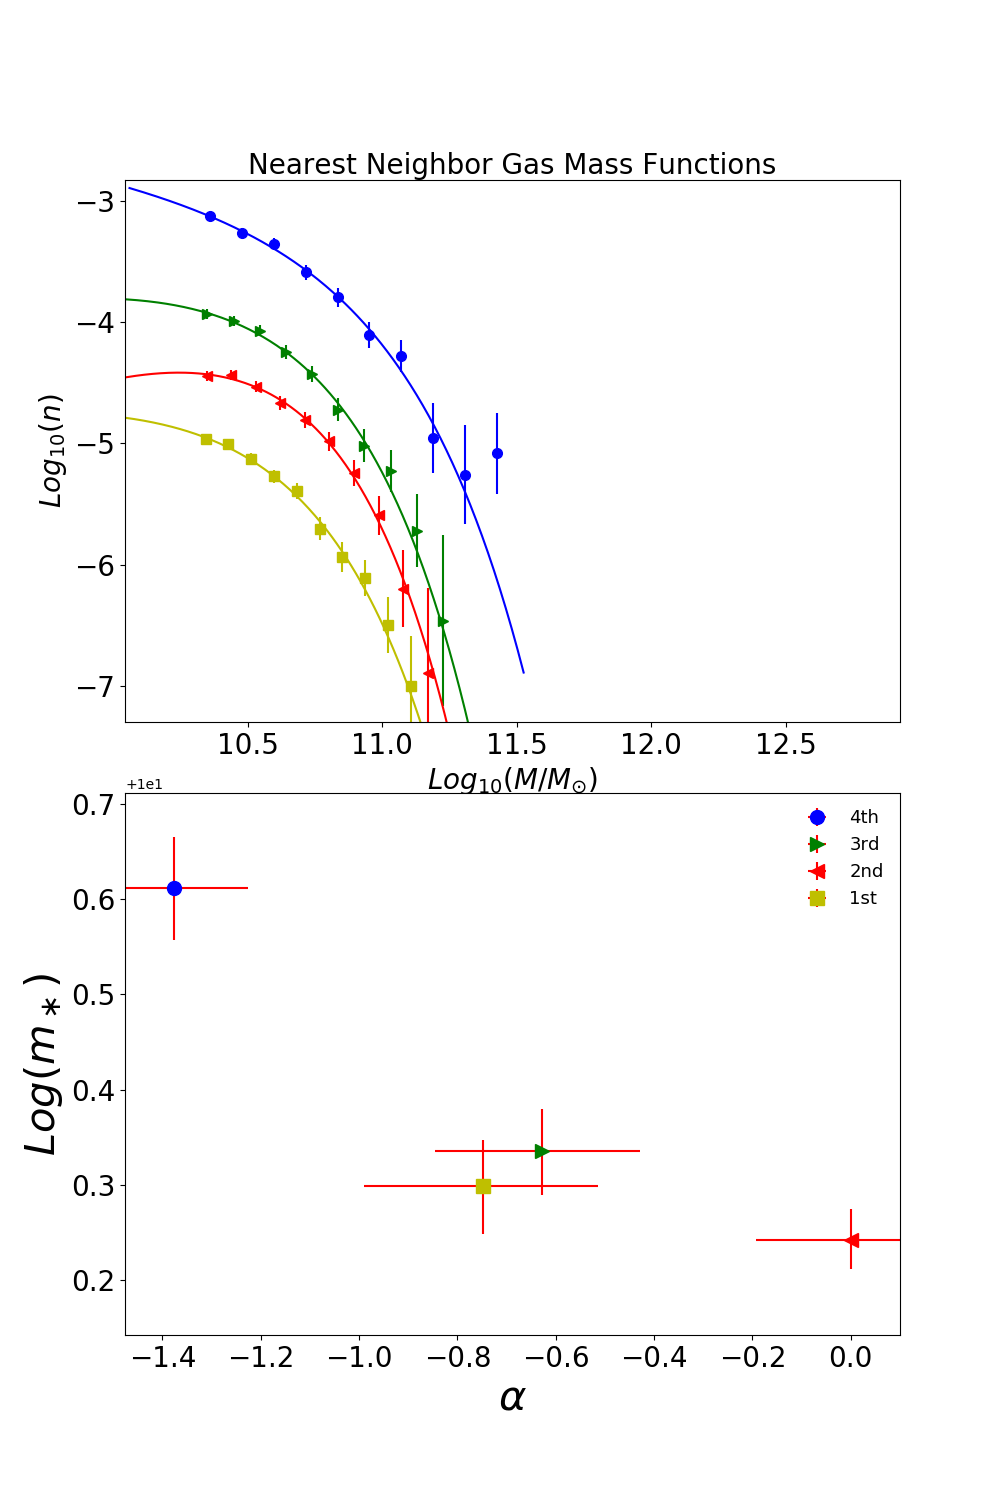
\includegraphics[width=\columnwidth]{./pics/F19_quartilesGas.png}
    \caption{\textbf{Upper side}: Schechter fits of each gas mass
      function for each environmental quartile (tendence) using the 3rd nearest
      neighbor definition.\textbf{Down side}: Knee-mass $m_\ast$ and
      the faint end slope $\alpha$ values obtained from the Schechter
      fits for each curve shown above.} 
    \label{fig:quartilesGas}
\end{figure}


% Quartiles Stellar
\begin{figure}
	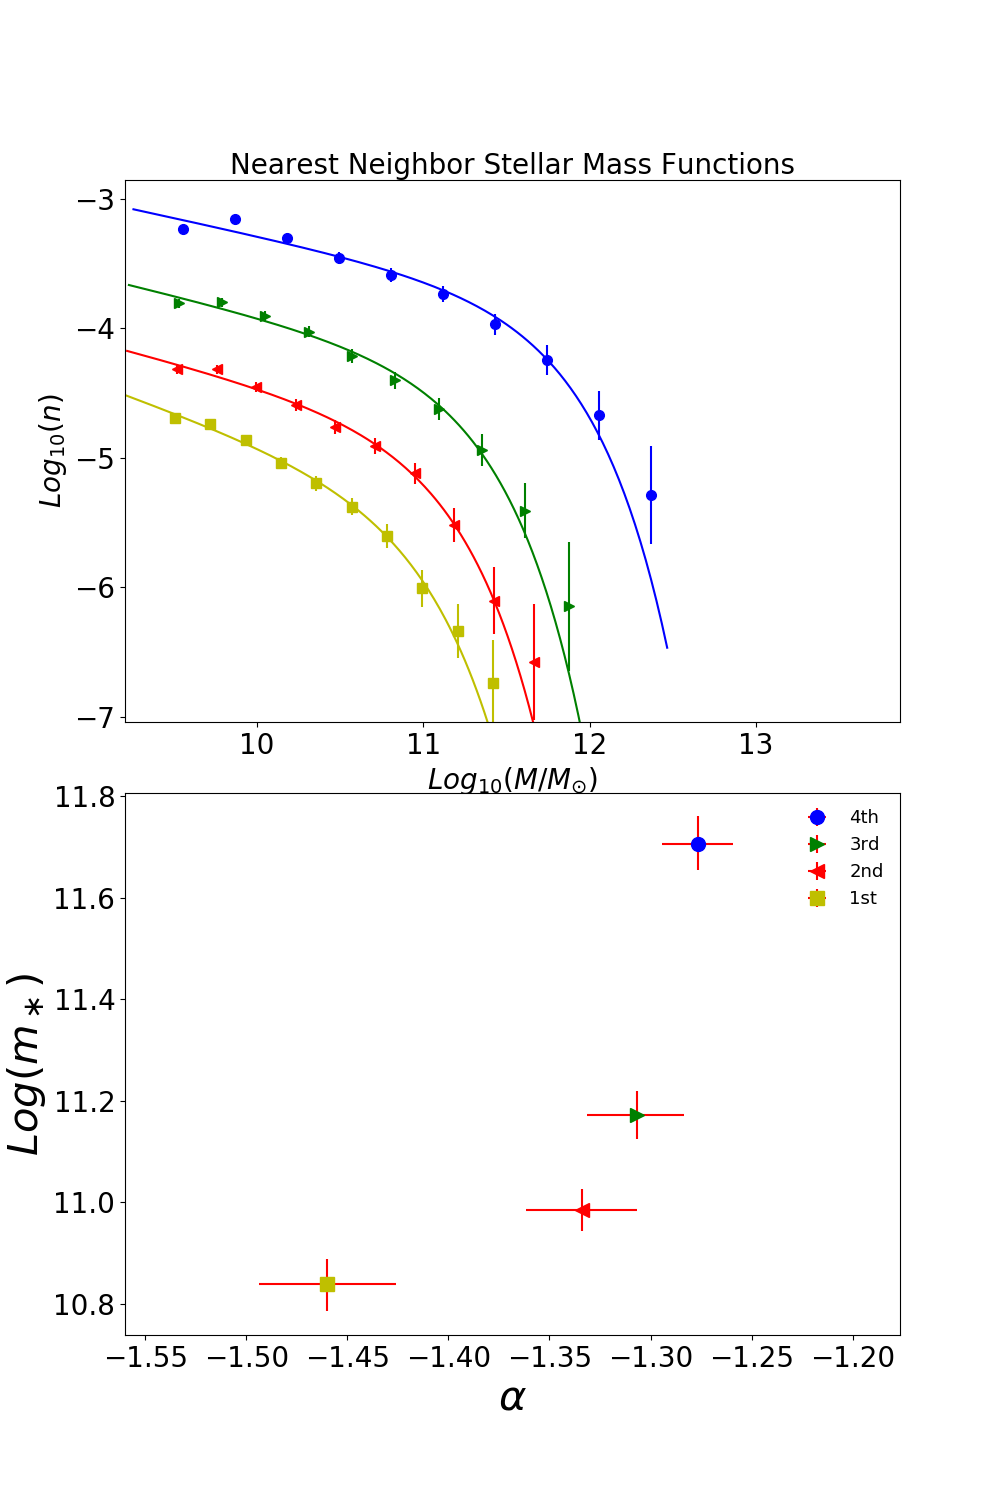
\includegraphics[width=\columnwidth]{./pics/F19_quartilesSellar.png}
    \caption{Similar to figure \ref{fig:quartilesGas} using stellar mass} 
    \label{fig:quartilesStellar}
\end{figure}


% Quartiles BH
\begin{figure}
	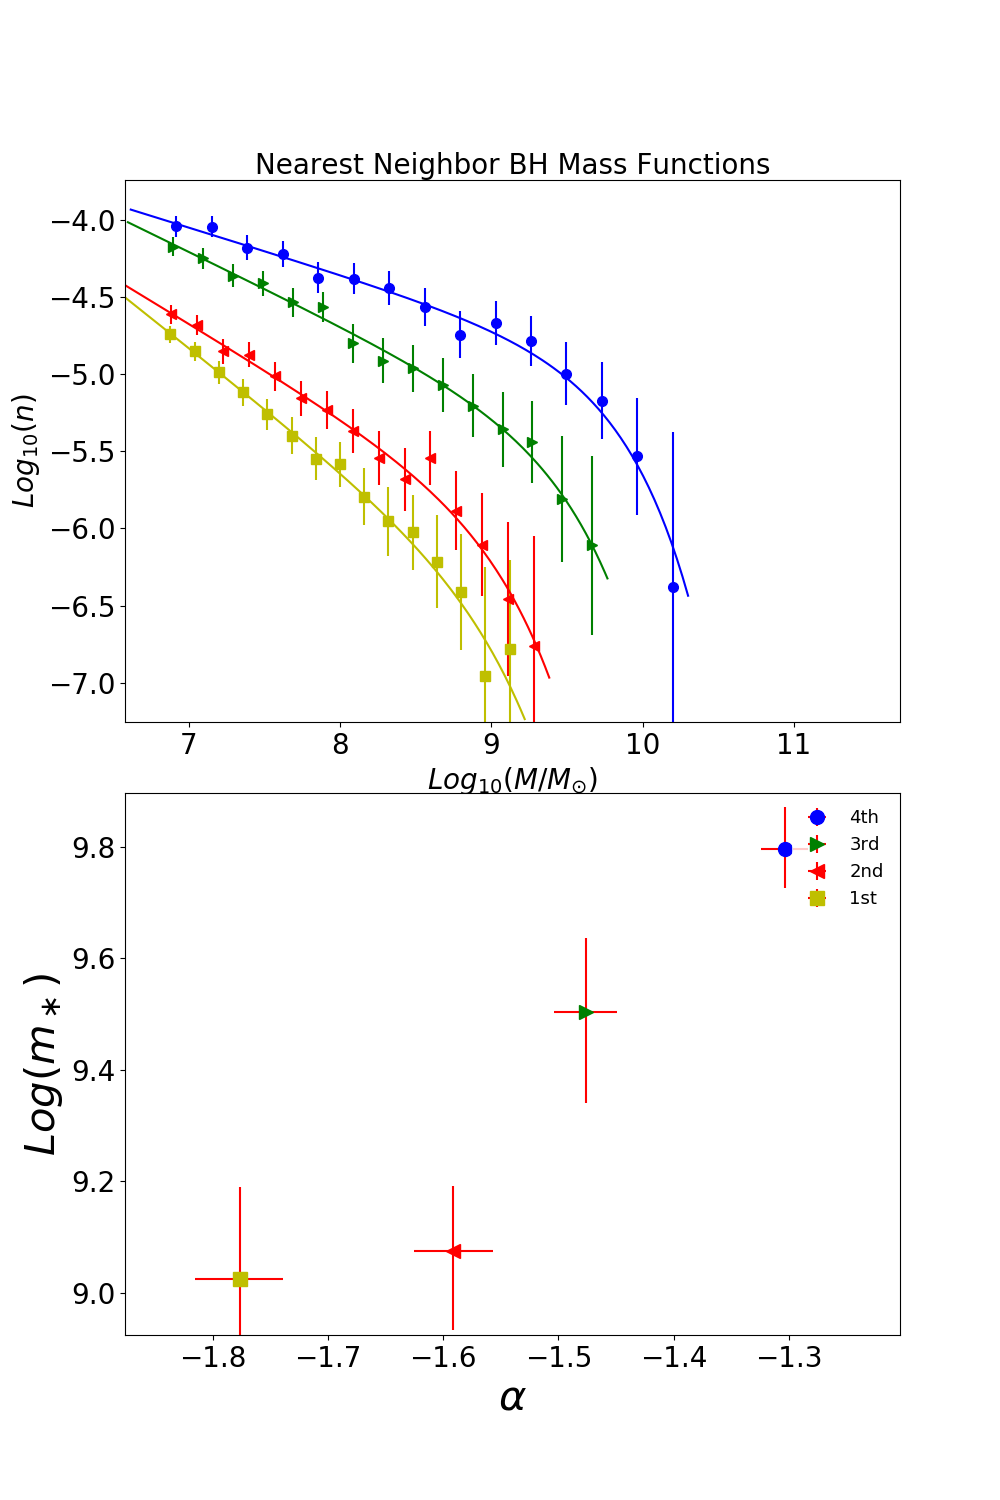
\includegraphics[width=\columnwidth]{./pics/F19_quartilesBH.png}
    \caption{Similar to figure \ref{fig:quartilesGas} using BHs mass.} 
    \label{fig:quartilesBH}
\end{figure}

% Quartiles DM
\begin{figure}
	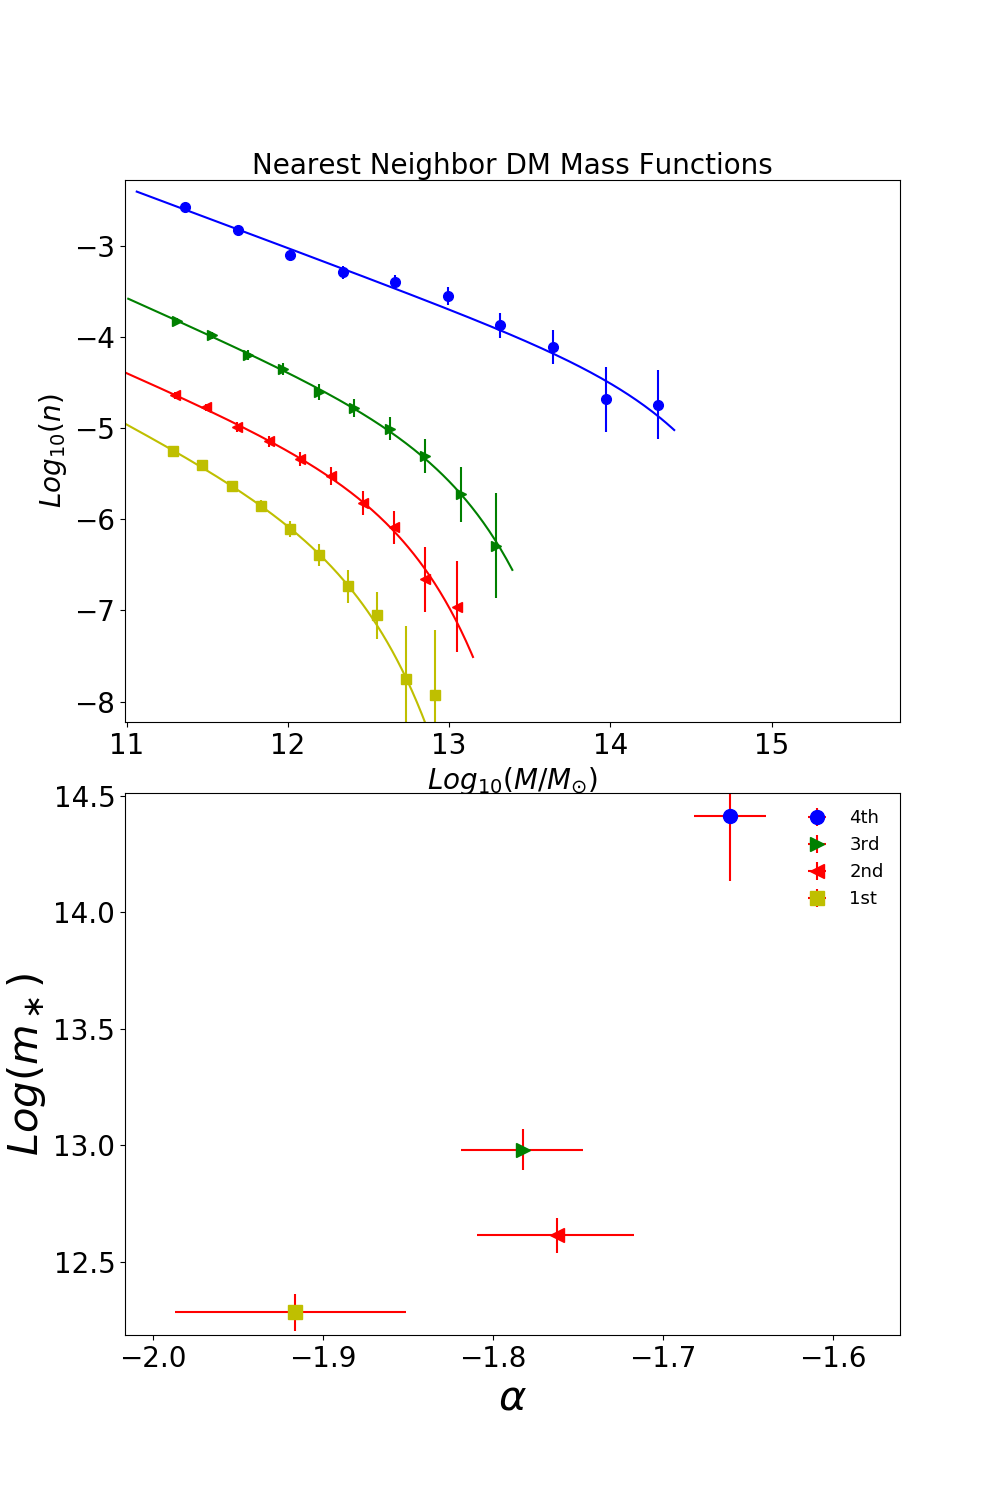
\includegraphics[width=\columnwidth]{./pics/F19_quartilesDM.png}
    \caption{Similar to figure \ref{fig:quartilesGas} using DM.} 
    \label{fig:quartilesDM}
\end{figure}



% Tweb gas
\begin{figure}
	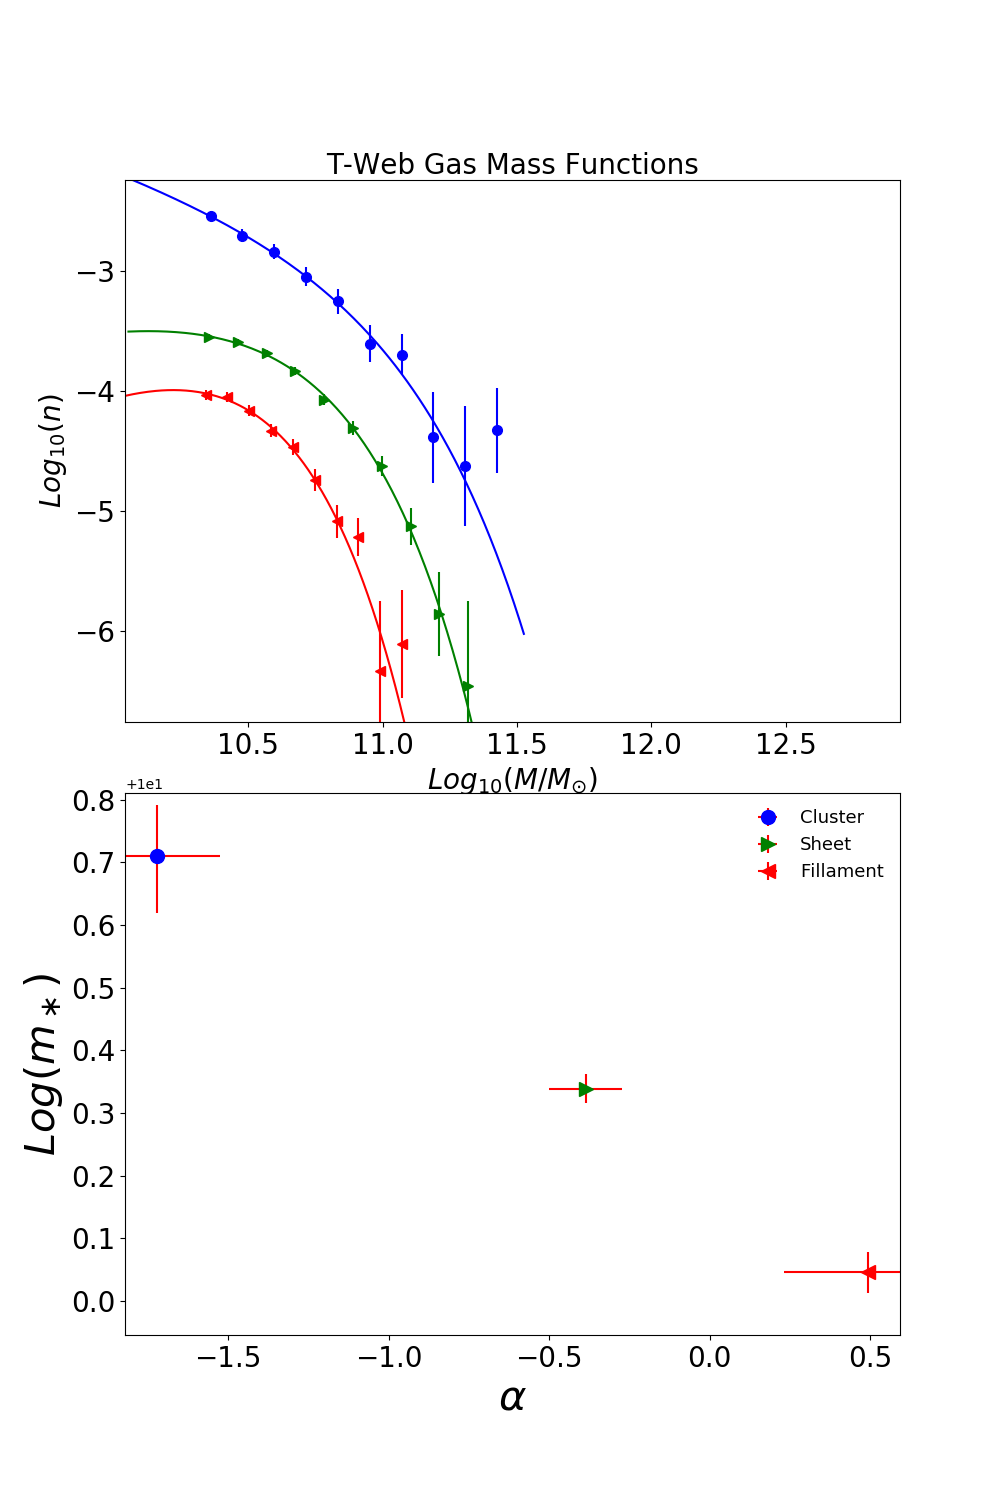
\includegraphics[width=\columnwidth]{./pics/F19_T-Web_Gas.png}
    \caption{\textbf{Upper side}: Schechter fits of each gas mass
      function for each morphological environment characterized by the
      T-Web algorithm proposed by Forero et al.\textbf{Down side}:
      Knee-mass $m_\ast$ and the faint end slope $\alpha$ values
      obtained from the Schechter fits for each curve shown above.} 
    \label{fig:TwebGas}
\end{figure}


% Tweb Stellar
\begin{figure}
	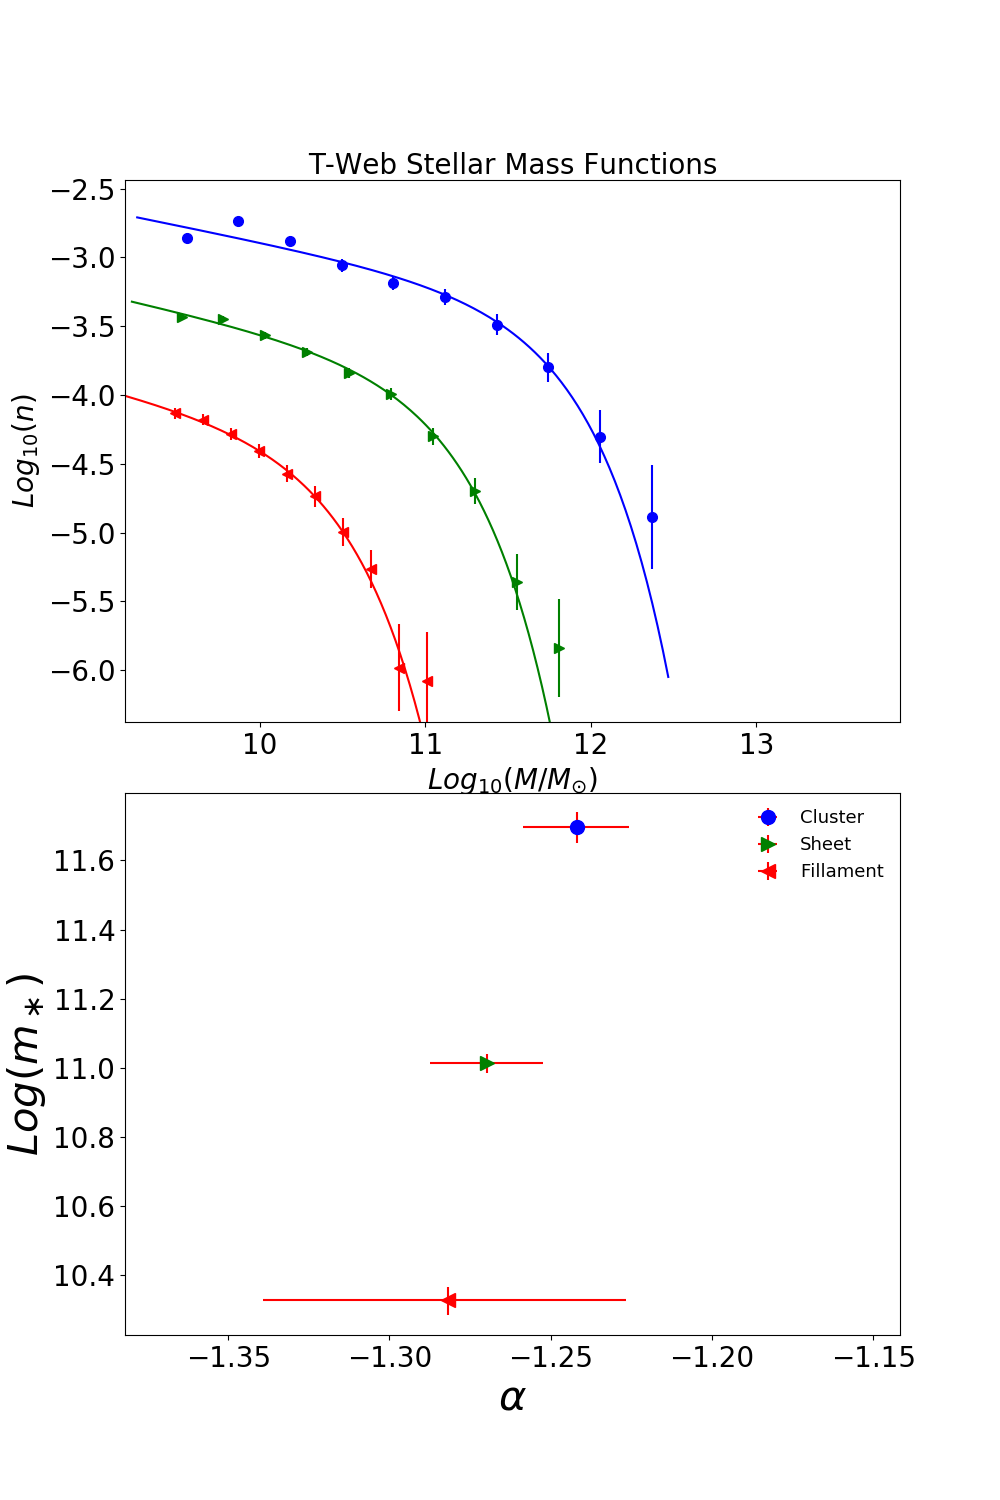
\includegraphics[width=\columnwidth]{./pics/F19_T-Web_Stellar.png}
    \caption{Similar to figure \ref{fig:TwebGas} using stellar mass} 
    \label{fig:TwebStellar}
\end{figure}


% Tweb BH
\begin{figure}
	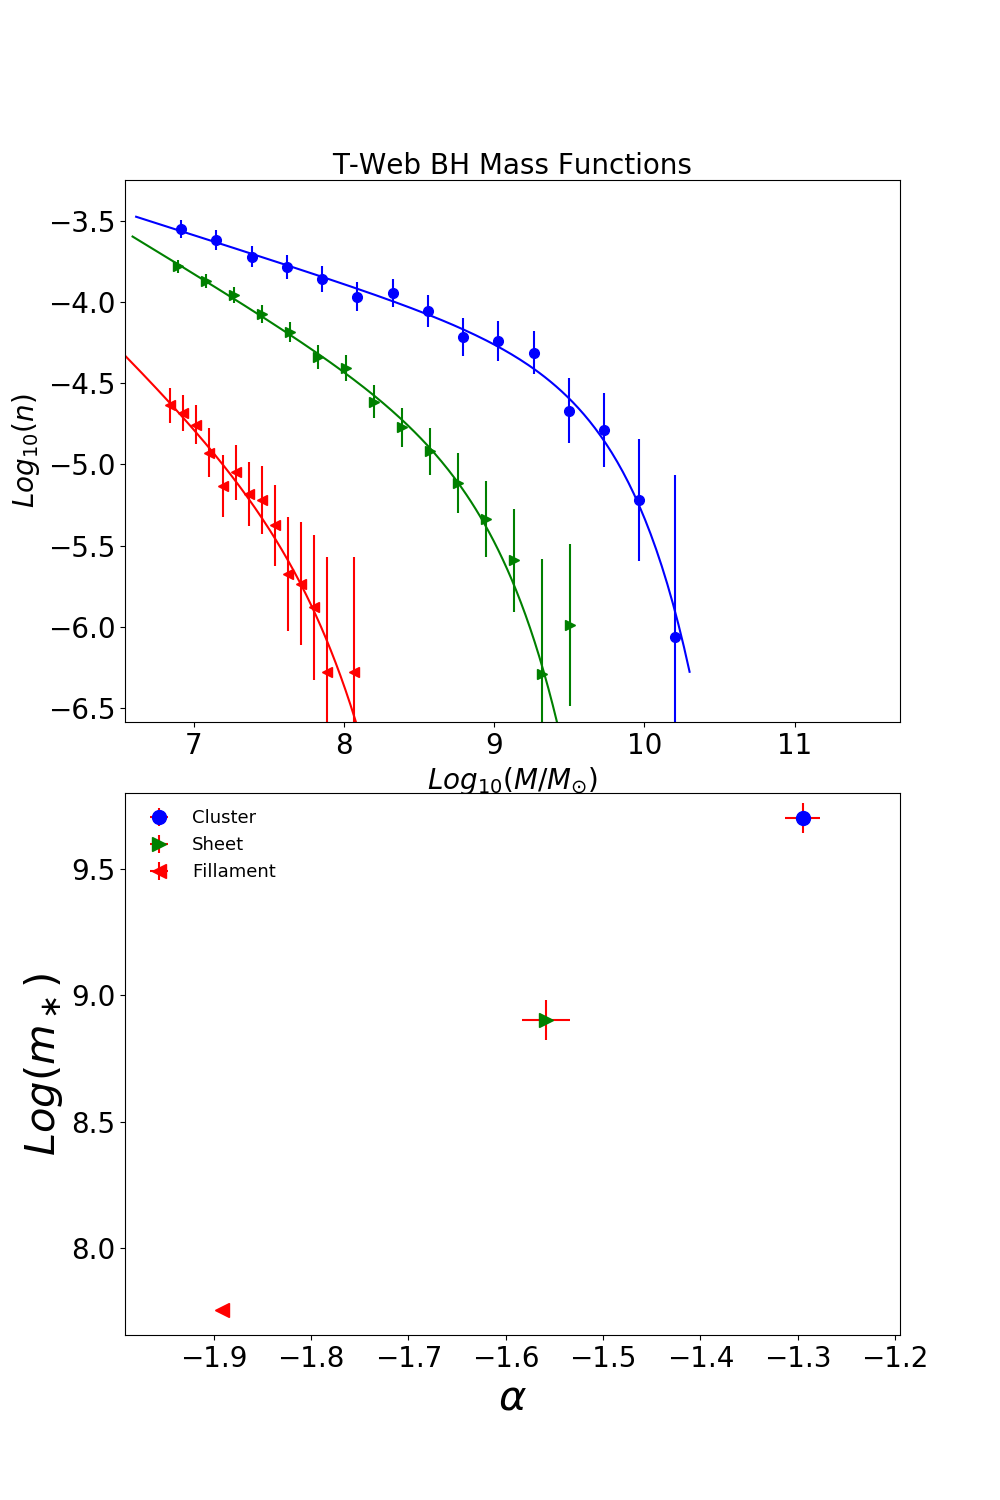
\includegraphics[width=\columnwidth]{./pics/F19_T-Web_BH.png}
    \caption{Similar to figure \ref{fig:TwebGas} using BHs mass.} 
    \label{fig:TwebBH}
\end{figure}



% Tweb DM
\begin{figure}
	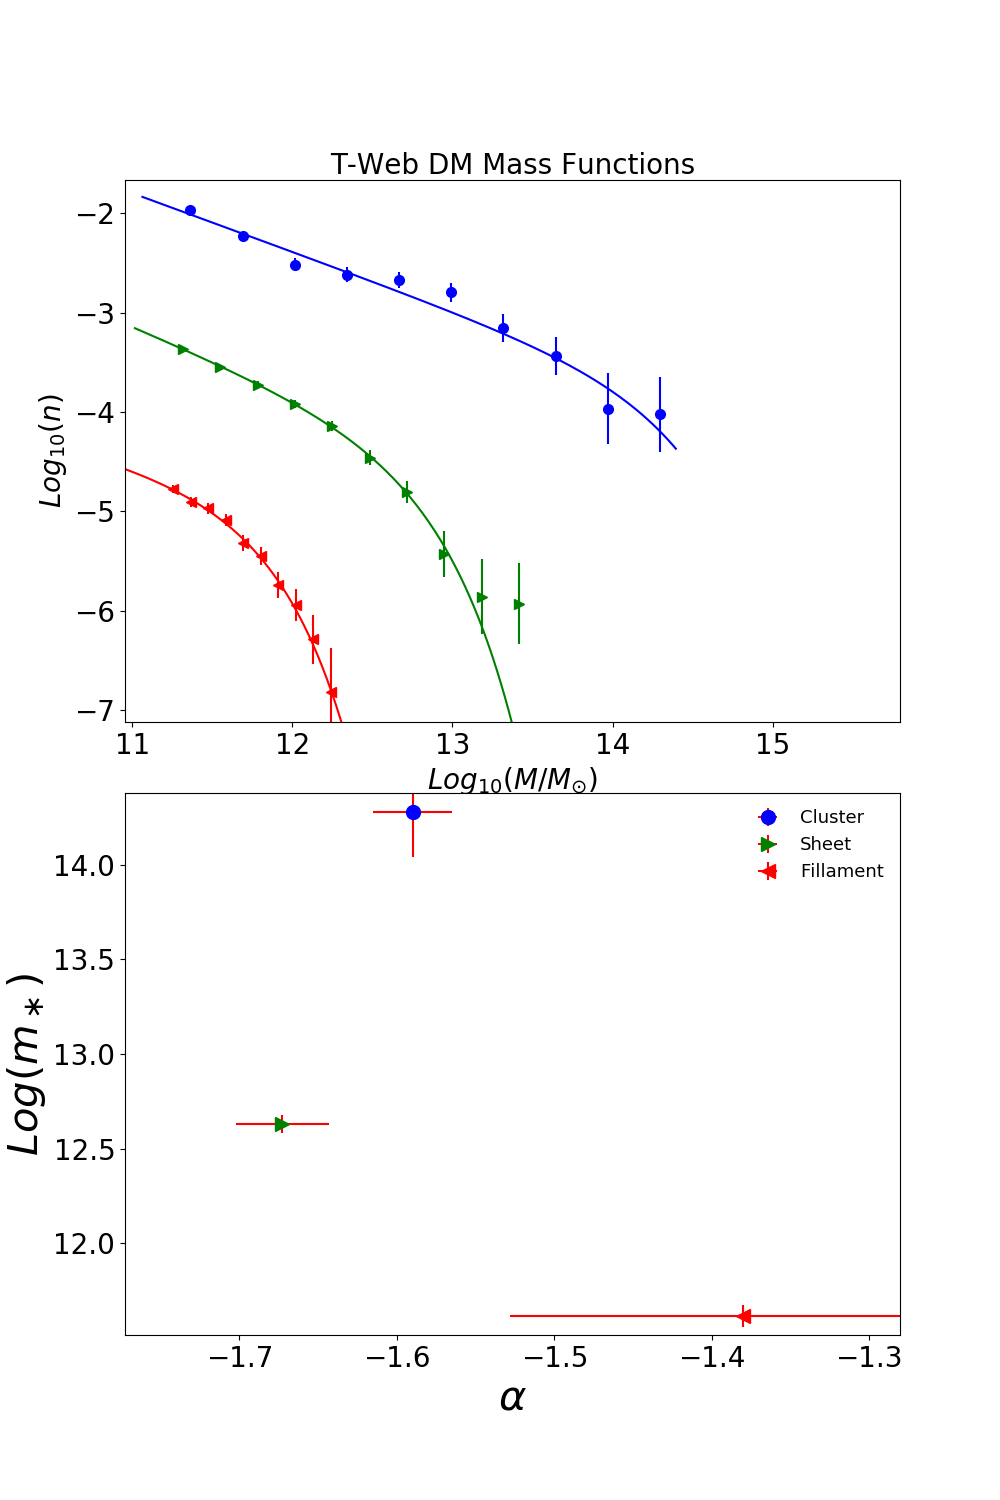
\includegraphics[width=\columnwidth]{./pics/F19_T-Web_DM.png}
    \caption{Similar to figure \ref{fig:TwebGas} using DM.} 
    \label{fig:TwebDM}
\end{figure}





\section{Conclusions}

The last numbered section should briefly summarise what has been done, and describe
the final conclusions which the authors draw from their work.

\section*{Acknowledgements}

The Acknowledgements section is not numbered. Here you can thank helpful
colleagues, acknowledge funding agencies, telescopes and facilities used etc.
Try to keep it short.

%%%%%%%%%%%%%%%%%%%%%%%%%%%%%%%%%%%%%%%%%%%%%%%%%%

%%%%%%%%%%%%%%%%%%%% REFERENCES %%%%%%%%%%%%%%%%%%

\bibliographystyle{mnras}
\bibliography{references}


%%%%%%%%%%%%%%%%%%%%%%%%%%%%%%%%%%%%%%%%%%%%%%%%%%


%%%%%%%%%%%%%%%%% APPENDICES %%%%%%%%%%%%%%%%%%%%%

\appendix

\section{Some extra material}

%%%%%%%%%%%%%%%%%%%%%%%%%%%%%%%%%%%%%%%%%%%%%%%%%%

\bsp	% typesetting comment
\label{lastpage}


\end{document}

% End of mnras_template.tex
